% !TeX program = lualatex
% ================================================================
% Polish Parallel Text Version of AlgebraNumberSenseStarters
%
% Generated by the server using the following settings:
%
%   language            Polish (pol)
%   text direction      left to right
%   font                Noto Serif
%   fallback font       Noto Serif
%   built from          latex/starters/targeted/KS3/algebra/algebraNumberSenseStarters.tex
%   vocabulary key      latex/starters/targeted/KS3/algebra/algebraNumberSenseStarters/L2/pol/algebraNumberSenseStarters_polishKey.tex
%   tier 3 vocabulary   green   RGB 0 128 0
%   English text        black   RGB 0 0 0
%   Polish text         purple  RGB 112 48 160
%   layout macros       version 3
%   sheet layout        version 1
%
% Please don't edit any information in this comment block - the server
% compares it against the current settings and rebuilds this file when
% they differ, so changes here would be overwritten. However, feel free
% to make updates to the LaTeX below if you want to edit it.
% ================================================================

\documentclass{beamer}
% ================================================================
% Copied from the English sheet this was translated from, so that
% anything it sets up for itself still works here
% ================================================================
\usepackage{tikz}
\usetikzlibrary{calc, arrows.meta, matrix, fit, shapes.geometric}
\usepackage{multicol}
\usepackage{amsmath}
\usepackage{amssymb}

% ================================================================
% Starters for a Year 7 class meeting algebra for the first time, used
% across the algebra unit.
%
% Each starter links an algebraic idea to the number work the class has
% already done, with decimals and negative numbers throughout. Most
% starters open with number calculations that the algebra later on the
% slide uses, and every starter has a sentence to complete with the
% words variable, term, coefficient, constant, expression, equation or
% solution. There are no bar models.
%
%   1  notation: what 3a, ab, a^2 and a/4 mean
%   2  substitution, with whole numbers, decimals and negative numbers
%   3  collecting like terms
%   4  multiplying and dividing terms, and powers
%   5  equations and their solutions, and one-step equations that add
%      or subtract
%   6  one-step equations that multiply or divide
%   7  two-step equations
%   8  two-step equations with decimals and negative numbers
%
% Starters 1 to 4 have no equations. Starters 5 to 8 build up to
% solving two-step equations, and each of them asks pupils to circle the
% reverse of an operation.
%
% The methods follow the ones the class was taught:
%   - Equations are solved by doing the same thing to both sides, never
%     with a flow chart. In the working, a curved arrow on each side goes
%     from one line of the equation to the next, with the operation
%     beside it. Starters 5 to 7 give the operations, and starter 8
%     leaves them blank.
%   - Bus stop division divides a decimal by a whole number, and
%     division by a decimal is done with equivalent fractions, for
%     example 6 / 0.5 = 60 / 5 = 12.
%
% The tables have their first entries filled in, as examples. An
% instruction that belongs to several questions has a bullet, and its
% questions are indented under it. The last question on each starter is
% a challenge, and in starters 1, 2 and 4 the challenge asks whether a
% statement is always, sometimes or never true.
% ================================================================

\setbeamertemplate{navigation symbols}{}
\setbeamersize{text margin left=0.4cm, text margin right=0.4cm}
\setlength{\multicolsep}{2pt}
\setlength{\columnsep}{20pt}

% ================================================================
% Answer-overlay helpers
% ================================================================
\newcommand{\ablank}[1]{%
  \alt<2>{\textcolor{red}{#1}}{\underline{\phantom{#1}}}%
}
\newcommand{\ashow}[1]{\uncover<2->{\textcolor{red}{\small #1}}}
\newcommand{\ashowq}[1]{\alt<2->{\textcolor{red}{\small #1}}{?}}

% Answers drawn straight on to a TikZ diagram, revealed on overlay 2 like \ashow.
% Space is reserved on overlay 1, so the diagram does not move between slides.
\usetikzlibrary{overlay-beamer-styles}
\tikzset{
  ans/.style     = {red, thick, visible on=<2->},
  ansfill/.style = {red!15, visible on=<2->},
  anslab/.style  = {red, font=\tiny, visible on=<2->},
}

% Used by the worked solutions rather than by this deck, so that each worked
% solution is first a question with room to write in and then the answer.
\newlength{\aworkpad}
\setlength{\aworkpad}{8mm}
\newcommand{\awork}[1]{%
  \par\vspace{\aworkpad}%
  \uncover<2->{#1}%
  \par\vspace{\aworkpad}%
}

% Every question list on these slides is tight, so that the diagram column and
% the question column both finish inside the slide.
\newcommand{\tightlist}{%
  \setlength{\itemsep}{0pt}\setlength{\parskip}{0pt}\setlength{\topsep}{0pt}%
}

% An instruction that belongs to several questions: \instr{Solve each
% equation.} puts it beside a bullet, where the question numbers go, and
% the questions in the subqs environment after it are indented under it.
% Their numbers carry on from the questions before them.
\setbeamertemplate{enumerate subitem}{\insertsubenumlabel.}
\renewcommand{\theenumii}{\arabic{enumii}}
\setbeamerfont{itemize/enumerate subbody}{size=\footnotesize}
\setlength{\leftmarginii}{1.4em}
\newcommand{\instr}[1]{%
  \item[{\usebeamercolor[fg]{itemize item}\usebeamertemplate{itemize item}}] #1}
\newenvironment{subqs}
  {\begin{enumerate}\tightlist\setcounter{enumii}{\value{enumi}}}
  {\setcounter{enumi}{\value{enumii}}\end{enumerate}}

% A temperature in degrees Celsius: \dC{-4}.
\newcommand{\dC}[1]{$#1\,^{\circ}$C}

% ================================================================
% The pictures these starters are built from.
% ================================================================
\tikzset{
  dhead/.style = {font=\scriptsize\bfseries, anchor=west},
  vans/.style  = {anslab, font=\scriptsize},
}

% A heading over a table or a picture in the diagram column.
\newcommand{\dheading}[1]{{\scriptsize\bfseries #1}\par\vspace{0.2em}}

% A blank in a table. It is never narrower than 1.6em, so that a one-digit
% answer still leaves a blank that can be seen. \tgiven is an entry that is
% filled in already, as an example, and is the same width.
\newcommand{\tblank}[1]{\ablank{\makebox[1.6em]{#1}}}
\newcommand{\tgiven}[1]{\makebox[1.6em]{#1}}

% Options to circle. \circleops{n}{k} writes +k, -k, \times k and \div k in a
% row, and circles the n-th of them in red on the answer slide. With k empty
% it writes the four signs on their own. The circle takes up no room in the
% line, so the options sit in the same places whichever one is circled, and
% the quads between them keep it clear of its neighbours.
\newcommand{\opt}[1]{\tikz[baseline=(o.base)]\node[inner sep=1.5pt, minimum width=1.6em] (o) {#1};}
\newcommand{\optc}[1]{\tikz[baseline=(o.base)]{%
  \node[inner sep=1.5pt, minimum width=1.6em] (o) {#1};
  \node[ans, draw, ellipse, inner sep=0pt, fit=(o), overlay] {};}}
\newcommand{\circleops}[2]{%
  \ifnum#1=1 \optc{$+#2$}\else\opt{$+#2$}\fi\quad
  \ifnum#1=2 \optc{$-#2$}\else\opt{$-#2$}\fi\quad
  \ifnum#1=3 \optc{$\times#2$}\else\opt{$\times#2$}\fi\quad
  \ifnum#1=4 \optc{$\div#2$}\else\opt{$\div#2$}\fi}

% Solving an equation by doing the same thing to both sides. The lines of the
% equation are the rows of a matrix, lined up on the equals sign, and a curved
% arrow on each side goes from one line to the next, with the operation beside
% it. The operations are a list, one for each step:
%   \bothsides{Working for Q6}{3n+4 \& = \& 19\\ 3n \& = \& \ablank{15}\\
%     n \& = \& \ablank{5}\\}{-4, \div3}
% An operation given as \ablank{...} is left for pupils to write in.
\tikzset{
  bsline/.style  = {matrix of math nodes, ampersand replacement=\&,
                    row sep=0.85em, column sep=0.15em,
                    nodes={inner sep=1pt, font=\footnotesize},
                    column 1/.style={anchor=base east},
                    column 2/.style={anchor=base},
                    column 3/.style={anchor=base west}},
  bsarrow/.style = {-{Stealth[length=3.5pt]}, blue!55!black, semithick},
  bslab/.style   = {font=\scriptsize, text=blue!55!black, inner sep=0.5pt},
}
\newcommand{\bothsides}[3]{%
  \par{\scriptsize\bfseries #1}\par\vspace{0.2em}%
  \begin{tikzpicture}[baseline=(current bounding box.north)]
    \matrix (m) [bsline] {#2};
    \foreach \op [count=\i, evaluate=\i as \j using int(\i+1)] in {#3} {
      \draw[bsarrow] ([xshift=-1pt]m.west |- m-\i-2.center) to[bend right=45]
        node[bslab, left] {$\op$} ([xshift=-1pt]m.west |- m-\j-2.center);
      \draw[bsarrow] ([xshift=1pt]m.east |- m-\i-2.center) to[bend left=45]
        node[bslab, right] {$\op$} ([xshift=1pt]m.east |- m-\j-2.center);
    }
  \end{tikzpicture}\par}

% ---- Bus stop division ----
% The dividend sits on the baseline y = 0 and the answer on y = 0.55, digit
% above digit, with the bus stop drawn between them. A remainder carried to
% the next digit is written small, just before that digit. \busframe{divisor}
% {right end} draws the divisor and the bus stop.
\tikzset{
  bsd/.style     = {font=\footnotesize, inner sep=0pt, anchor=base},
  bsa/.style     = {bsd, red, visible on=<2->},
  bscarry/.style = {font=\tiny, inner sep=0pt, anchor=base, red, visible on=<2->},
}
\newcommand{\busframe}[2]{%
  \node[bsd, anchor=base east] at (-0.1,0) {$#1$};
  \draw[thick] (0,-0.12) -- (0,0.4) -- (#2,0.4);}

% \rect{length}{width}{label in the middle}: a rectangle 2.5 cm by 1.1 cm,
% with its length written above it and its width to its left.
\newcommand{\rect}[3]{%
  \draw[thick, fill=blue!6] (0.9,0) rectangle (3.4,1.1);
  \node[above] at (2.15,1.1) {$#1$};
  \node[left] at (0.9,0.55) {$#2$};
  \node at (2.15,0.55) {#3};}

\title{Algebra \& Number Sense: Starters}
\author{}
\date{}

% Characters this language's font has not got are borrowed from another,
% rather than being silently dropped - see docs/translated-sheet-latex.md
\directlua{%
  if luaotfload and luaotfload.add_fallback then
    luaotfload.add_fallback("eallatinfallback",
      { "Noto Serif:mode=harf;" })
  else
    tex.error("this luaotfload is too old to register a fallback font")
  end
}
\usepackage[english]{babel}
\babelprovide[import]{polish}
\babelfont[polish]{rm}[Renderer=Harfbuzz, BoldFont={Noto Serif}, ItalicFont={Noto Serif}, BoldItalicFont={Noto Serif}, RawFeature={fallback=eallatinfallback}]{Noto Serif}
\babelfont[polish]{sf}[Renderer=Harfbuzz, BoldFont={Noto Serif}, ItalicFont={Noto Serif}, BoldItalicFont={Noto Serif}, RawFeature={fallback=eallatinfallback}]{Noto Serif}
\newcommand{\ealtext}[1]{\foreignlanguage{polish}{#1}}
\newcommand{\ealtextblock}[1]{{\raggedright\foreignlanguage{polish}{#1}\par}}
% ================================================================
% EAL layout helpers
% ================================================================
\usepackage{xcolor}

\definecolor{ealkeycolour}{RGB}{0,128,0}
\definecolor{ealenglish}{RGB}{0,0,0}
\definecolor{ealtwocolour}{RGB}{112,48,160}

\newsavebox{\ealboxen}
\newsavebox{\ealboxtr}
\newlength{\ealglosswd}
\newlength{\ealglossraise}
\setlength{\ealglossraise}{1.15em}

% a tier 3 word, in English and in translation alike
\newcommand{\ealkey}[1]{\textcolor{ealkeycolour}{#1}}
\newcommand{\ealkeytr}[1]{\textcolor{ealkeycolour}{\ealtext{#1}}}

% One translated word above one English word. Built from kernel
% primitives, never a tabular, which would break wherever the sheet
% loads array, booktabs or tabularx. The box is as wide as the wider of
% the two, so a long translation pushes its neighbours aside instead of
% overlapping them, and it claims its full height so a table row or a
% TikZ node makes room for it.
\newcommand{\ealgloss}[2]{%
  \sbox{\ealboxen}{\ealkey{#1}}%
  \sbox{\ealboxtr}{\small\textcolor{ealtwocolour}{\ealtext{#2}}}%
  \setlength{\ealglosswd}{\wd\ealboxen}%
  \ifdim\wd\ealboxtr>\ealglosswd\setlength{\ealglosswd}{\wd\ealboxtr}\fi
  \leavevmode
  \makebox[\ealglosswd][c]{%
    \makebox[0pt][c]{\usebox{\ealboxen}}%
    \makebox[0pt][c]{\raisebox{\ealglossraise}{\usebox{\ealboxtr}}}%
  }%
}

% opens up line spacing around a block of glosses, so the raised
% translations sit clear of the line above
\newenvironment{ealglossed}{\par\linespread{2.1}\selectfont\ignorespaces}{\par}

% a whole translated sentence above its English counterpart. block level,
% so it does not belong inside a tabular cell
\newcommand{\ealpara}[2]{%
  \par\addvspace{0.5\baselineskip}%
  {\color{ealtwocolour}\ealtextblock{#1}}%
  \penalty200
  {\color{ealenglish}#2\par}%
  \addvspace{0.5\baselineskip}%
}

\begin{document}

\frame{\titlepage}

\begin{frame}[t]{Starter 1: \ealkey{Algebraic Notation} (1 of 3)}
\footnotesize
\begin{enumerate}\setcounter{enumi}{0}\tightlist
\begin{multicols}{2}
  \item $3\times(-2)=$\ashow{$-6$}
  \columnbreak
  \item $3\times0.4=$\ashow{$1.2$}
\end{multicols}
\end{enumerate}
\end{frame}

\begin{frame}[t]{Starter 1: \ealkey{Algebraic Notation} (2 of 3)}
\begin{columns}[T,onlytextwidth]
\column{0.32\textwidth}
\vspace{-0.4em}
\dheading{Table for Q3}
{\footnotesize
\renewcommand{\arraystretch}{1.25}
\begin{tabular}{@{}l|l@{}}
  With $\times$ or $\div$ & In \ealkey{algebra}\\ \hline
  $3\times a$ & \tgiven{$3a$}\\
  $a\times b$ & \tblank{$ab$}\\
  $a\times a$ & \tblank{$a^2$}\\
  $a\div4$    & \tblank{$\dfrac{a}{4}$}\\[2pt]
  $1\times a$ & \tblank{$a$}
\end{tabular}}

\column{0.68\textwidth}
\vspace{-1.5em}
\footnotesize
\begin{enumerate}\setcounter{enumi}{2}\tightlist
  \item \ealpara{Zapisz każde z nich w \ealkeytr{algebrze}, w tabeli po lewej. Pierwsze jest już zrobione za ciebie.}{Write each one in \ealkey{algebra}, in the table on the left. The first one is done for you.}
  \ealpara{Znajdź \ealkeytr{wartość} $3a$:}{}
  \instr{Find the \ealkey{value} of $3a$:}
  \begin{subqs}
  {\setlength{\columnsep}{12pt}%
  \begin{multicols}{3}
    \item \ealpara{gdy $a=5$}{when $a=5$} \ashow{$15$, not $35$}
    \columnbreak
    \item \ealpara{gdy $a=0.4$}{when $a=0.4$} \ashow{$1.2$}
    \columnbreak
    \item \ealpara{gdy $a=-2$}{when $a=-2$} \ashow{$-6$}
  \end{multicols}}
  \end{subqs}
  \item \ealpara{W $7y+2$, $7$ jest \ablank{\ealkeytr{współczynnikiem}}, $y$ jest \ablank{\ealkeytr{zmienną}}, a $2$ jest \ablank{\ealkeytr{stałą}}.}{In $7y+2$, the $7$ is the \ablank{\ealkey{coefficient}}, $y$ is the \ablank{\ealkey{variable}} and $2$ is the \ablank{\ealkey{constant}}.}
  \ealpara{Zapisz \ealkeytr{wyrażenie} dla każdego z nich.}{}
  \instr{Write an \ealkey{expression} for each one.}
  \begin{subqs}
  \begin{multicols}{2}
    \item \ealpara{$n$ pomnożone przez $4$, następnie dodane $3$}{$n$ multiplied by $4$, then $3$ added} \ashow{$4n+3$}
    \columnbreak
    \item \ealpara{$n$ podzielone przez $2$, następnie odjęte $1$}{$n$ divided by $2$, then $1$ subtracted} \ashow{$\tfrac{n}{2}-1$}
  \end{multicols}
  \end{subqs}
\end{enumerate}
\end{columns}
\end{frame}

\begin{frame}[t]{Starter 1: \ealkey{Algebraic Notation} (3 of 3)}
\footnotesize
\begin{enumerate}\setcounter{enumi}{4}\tightlist
  \item \ealpara{Czy każde stwierdzenie jest zawsze, czasami czy nigdy prawdziwe? Wypróbuj kilka \ealkeytr{wartości} $a$ i $b$.}{}
  \instr{Is each statement always, sometimes or never true? Try some \ealkey{values} of $a$ and $b$.}
  \begin{subqs}
    \item \ealpara{(Wyzwanie) $ab$ i $ba$ mają tę samą \ealkeytr{wartość}.}{(Challenge) $ab$ and $ba$ have the same \ealkey{value}.} \ashow{Always, for example $5\times3=3\times5$.}
    \item \ealpara{(Wyzwanie) $a-b$ i $b-a$ mają tę samą \ealkeytr{wartość}.}{(Challenge) $a-b$ and $b-a$ have the same \ealkey{value}.} \ashow{Sometimes: only when $a=b$, because $5-3=2$ but $3-5=-2$.}
  \end{subqs}
\end{enumerate}
\end{frame}

\begin{frame}[t]{Starter 2: \ealkey{Substitution} (1 of 3)}
\footnotesize
\begin{enumerate}\setcounter{enumi}{0}\tightlist
\begin{multicols}{2}
  \item $5-(-2)=$\ashow{$7$}
  \columnbreak
  \item $4\times(-3)=$\ashow{$-12$}
\end{multicols}
  \item \ealpara{Zastępowanie \ealkeytr{zmiennej} liczbą nazywa się \ealkeytr{podstawieniem}.}{Replacing a \ealkey{variable} with a number is called \ealkey{substitution}.}
\end{enumerate}
\end{frame}

\begin{frame}[t]{Starter 2: \ealkey{Substitution} (2 of 3)}
\begin{columns}[T,onlytextwidth]
\column{0.32\textwidth}
\vspace{-0.4em}
\dheading{Table for Q4}
{\footnotesize
\renewcommand{\arraystretch}{1.3}\setlength{\tabcolsep}{4pt}
\begin{tabular}{@{}c|c|c|c@{}}
  $x$   & $2x$ & $x+3$ & $5-x$\\ \hline
  $4$   & \tgiven{$8$}  & \tgiven{$7$}   & \tblank{$1$}\\
  $0.5$ & \tblank{$1$}  & \tblank{$3.5$} & \tgiven{$4.5$}\\
  $-2$  & \tblank{$-4$} & \tblank{$1$}   & \tblank{$7$}
\end{tabular}}

\column{0.68\textwidth}
\vspace{-1.5em}
\footnotesize
\begin{enumerate}\setcounter{enumi}{3}\tightlist
  \item \ealpara{Uzupełnij tabelę po lewej. Trzy odpowiedzi są już zrobione za ciebie.}{Complete the table on the left. Three of the answers are done for you.}
  \ealpara{Znajdź \ealkeytr{wartość} $4a-1$:}{}
  \instr{Find the \ealkey{value} of $4a-1$:}
  \begin{subqs}
  \begin{multicols}{2}
    \item \ealpara{gdy $a=3$}{when $a=3$} \ashow{$12-1=11$}
    \columnbreak
    \item \ealpara{gdy $a=-3$}{when $a=-3$} \ashow{$-12-1=-13$}
  \end{multicols}
  \end{subqs}
  \item \ealpara{Znajdź \ealkeytr{wartość} $3x^2$, gdy $x=2$.}{Find the \ealkey{value} of $3x^2$ when $x=2$.}
        \ashow{$3\times4=12$. The \ealkey{power} comes first, so it is not $6^2$.}
  \item \ealpara{Podróż taksówką o długości $m$ mil kosztuje \pounds$(2.5m+3)$. Ile kosztuje podróż o długości $4$ mil?}{A taxi journey of $m$ miles costs \pounds$(2.5m+3)$. How much does a $4$ mile journey cost?}
        \ashow{$2.5\times4+3=13$, so \pounds13}
\end{enumerate}
\end{columns}
\end{frame}

\begin{frame}[t]{Starter 2: \ealkey{Substitution} (3 of 3)}
\footnotesize
\begin{enumerate}\setcounter{enumi}{6}\tightlist
  \item \ealpara{W $2.5m+3$, \ealkeytr{współczynnik} $m$ wynosi \ablank{$2.5$}, a \ealkeytr{stała} wynosi \ablank{$3$}.}{In $2.5m+3$, the \ealkey{coefficient} of $m$ is \ablank{$2.5$} and the \ealkey{constant} is \ablank{$3$}.}
  \item \ealpara{(Wyzwanie) Czy to stwierdzenie jest zawsze, czasami czy nigdy prawdziwe? $2x$ jest większe niż $x$.}{(Challenge) Is this statement always, sometimes or never true? $2x$ is bigger than $x$.}
        \ashow{Sometimes. It is true when $x$ is \ealkey{positive}, but when $x=-1$, $2x=-2$.}
\end{enumerate}
\end{frame}

\begin{frame}[t]{Starter 3: \ealkey{Collecting} \ealkey{Like Terms} (1 of 3)}
\footnotesize
\begin{enumerate}\setcounter{enumi}{0}\tightlist
  \item \ealpara{Wykonaj każde obliczenie, a następnie użyj go, aby \ealkeytr{uprościć} \ealkeytr{wyrażenie} obok.}{}
  \instr{Work out each calculation, then use it to \ealkey{simplify} the \ealkey{expression} beside it.}
  \begin{subqs}
  \begin{multicols}{2}
    \item $-2+5=$\ashow{$3$}
    \item $4-9=$\ashow{$-5$}
    \item $0.3+0.4=$\ashow{$0.7$}
    \columnbreak
    \item $-2a+5a=$\ashow{$3a$}
    \item $4y-9y=$\ashow{$-5y$}
    \item $0.3x+0.4x=$\ashow{$0.7x$}
  \end{multicols}
  \end{subqs}
  \item \ealpara{$3x$ i $4x$ nazywamy \ablank{\ealkeytr{wyrazami podobnymi}}, ponieważ różnią się tylko \ablank{\ealkeytr{współczynnikami}}.}{$3x$ and $4x$ are called \ablank{\ealkey{like terms}}, because only their \ablank{\ealkey{coefficients}} are different.}
  \ealpara{Uprość każde \ealkeytr{wyrażenie}.}{}
  \instr{\ealkey{Simplify} each \ealkey{expression}.}
  \begin{subqs}
  \begin{multicols}{2}
    \item $5a+2b-3a+b=$\ashow{$2a+3b$}
    \columnbreak
    \item $1.5m-4+2.5m+6=$\ashow{$4m+2$}
  \end{multicols}
  \end{subqs}
\end{enumerate}
\end{frame}

\begin{frame}[t]{Starter 3: \ealkey{Collecting} \ealkey{Like Terms} (2 of 3)}
\begin{columns}[T,onlytextwidth]
\column{0.32\textwidth}
\vspace{-0.4em}
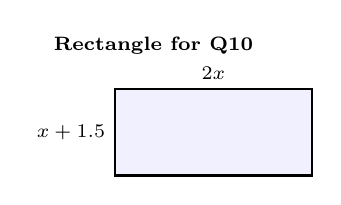
\begin{tikzpicture}[every node/.style={font=\scriptsize}]
\node[dhead] at (0,1.65) {Rectangle for Q10};
\rect{2x}{x+1.5}{}
\end{tikzpicture}

\column{0.68\textwidth}
\vspace{-1.5em}
\footnotesize
\begin{enumerate}\setcounter{enumi}{2}\tightlist
  \item \ealpara{Zapisz \ealkeytr{wyrażenie} na \ealkeytr{obwód} \ealkeytr{prostokąta} i je \ealkeytr{uprość}.}{Write an \ealkey{expression} for the \ealkey{perimeter} of the \ealkey{rectangle}, and \ealkey{simplify} it.}
        \ashow{$2x+2x+(x+1.5)+(x+1.5)=6x+3$}
  \item \ealpara{Ali \ealkeytr{upraszcza} $3x+4y$ do $7xy$. Sprawdź to za pomocą $x=2$ i $y=10$.}{Ali \ealkey{simplifies} $3x+4y$ to $7xy$. Test this with $x=2$ and $y=10$.}
        \ashow{$3x+4y=6+40=46$, but $7xy=140$}
\end{enumerate}
\end{columns}
\end{frame}

\begin{frame}[t]{Starter 3: \ealkey{Collecting} \ealkey{Like Terms} (3 of 3)}
\footnotesize
\begin{enumerate}\setcounter{enumi}{4}\tightlist
  \item \ealpara{(Wyzwanie) Zapisz \ealkeytr{wyrażenie} z czterema \ealkeytr{wyrazami}, które \ealkeytr{upraszcza} się do $-3x+0.5$.}{(Challenge) Write an \ealkey{expression} with four \ealkey{terms} that \ealkey{simplifies} to $-3x+0.5$.}
        \ashow{For example $x-4x+1-0.5$}
\end{enumerate}
\end{frame}

\begin{frame}[t]{Starter 4: Multiplying \ealkey{Terms} \& \ealkey{Powers} (1 of 3)}
\footnotesize
\begin{enumerate}\setcounter{enumi}{0}\tightlist
  \item \ealpara{Wykonaj każde obliczenie, a następnie użyj go, aby \ealkeytr{uprościć} \ealkeytr{wyrażenie} obok.}{}
  \instr{Work out each calculation, then use it to \ealkey{simplify} the \ealkey{expression} beside it.}
  \begin{subqs}
  \begin{multicols}{2}
    \item $-4\times3=$\ashow{$-12$}
    \item $0.5\times0.5=$\ashow{$0.25$}
    \columnbreak
    \item $-4\times3a=$\ashow{$-12a$}
    \item $0.5a\times0.5a=$\ashow{$0.25a^2$}
  \end{multicols}
  \end{subqs}
  \item \ealpara{W $0.25a^2$, $0.25$ jest \ablank{\ealkeytr{współczynnikiem}}, a $2$ jest \ablank{\ealkeytr{potęgą}}.}{In $0.25a^2$, the $0.25$ is the \ablank{\ealkey{coefficient}} and the $2$ is the \ablank{\ealkey{power}}.}
  \item \ealpara{Uprość każde \ealkeytr{wyrażenie}.}{}
  \instr{\ealkey{Simplify} each \ealkey{expression}.}
  \begin{subqs}
  \begin{multicols}{2}
    \item $4x\times x=$\ashow{$4x^2$}
    \columnbreak
    \item $-12a\div4=$\ashow{$-3a$}
  \end{multicols}
  \end{subqs}
\end{enumerate}
\end{frame}

\begin{frame}[t]{Starter 4: Multiplying \ealkey{Terms} \& \ealkey{Powers} (2 of 3)}
\begin{columns}[T,onlytextwidth]
\column{0.32\textwidth}
\vspace{-0.4em}
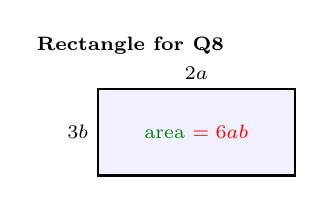
\begin{tikzpicture}[every node/.style={font=\scriptsize}]
\node[dhead] at (0,1.65) {Rectangle for Q8};
\rect{2a}{3b}{}
\node[vans] at (2.15,0.55) {\ealkey{area} $=6ab$};
\end{tikzpicture}

\vspace{1.2em}
\dheading{Table for Q9}
{\footnotesize
\renewcommand{\arraystretch}{1.3}\setlength{\tabcolsep}{4pt}
\begin{tabular}{@{}c|c|c|c|c@{}}
  $a$   & $3$ & $1$ & $0.5$ & $-2$\\ \hline
  $a^2$ & \tgiven{$9$} & \tblank{$1$} & \tblank{$0.25$} & \tblank{$4$}
\end{tabular}}

\column{0.68\textwidth}
\vspace{-1.5em}
\footnotesize
\begin{enumerate}\setcounter{enumi}{3}\tightlist
  \item \ealpara{Zapisz \ealkeytr{wyrażenie} na \ealkeytr{pole} \ealkeytr{prostokąta}. Znajdź \ealkeytr{pole}, gdy $a=1.5$ i $b=2$.}{Write an \ealkey{expression} for the \ealkey{area} of the \ealkey{rectangle}. Find the \ealkey{area} when $a=1.5$ and $b=2$.}
        \ashow{$2a\times3b=6ab$, \; $6\times1.5\times2=18$}
  \item \ealpara{Uzupełnij tabelę. Pierwsze jest już zrobione za ciebie. Dla której \ealkeytr{wartości} $a$ jest $a^2$ mniejsze niż $a$?}{Complete the table. The first one is done for you. For which \ealkey{value} of $a$ is $a^2$ smaller than $a$?}
        \ashow{$a=0.5$}
\end{enumerate}
\end{columns}
\end{frame}

\begin{frame}[t]{Starter 4: Multiplying \ealkey{Terms} \& \ealkey{Powers} (3 of 3)}
\footnotesize
\begin{enumerate}\setcounter{enumi}{5}\tightlist
  \item \ealpara{Znajdź \ealkeytr{wartość} każdego \ealkeytr{wyrażenia}, gdy $a=3$.}{}
  \instr{Find the \ealkey{value} of each \ealkey{expression} when $a=3$.}
  \begin{subqs}
  \begin{multicols}{2}
    \item $2a^2=$\ashow{$2\times9=18$}
    \columnbreak
    \item $(2a)^2=$\ashow{$6^2=36$}
  \end{multicols}
  \end{subqs}
  \item \ealpara{(Wyzwanie) Czy to stwierdzenie jest zawsze, czasami czy nigdy prawdziwe? $a^2$ jest większe niż $a$.}{(Challenge) Is this statement always, sometimes or never true? $a^2$ is bigger than $a$.}
        \ashow{Sometimes. It is not true when $a$ is from $0$ to $1$, for example $0.5^2=0.25$.}
\end{enumerate}
\end{frame}

\begin{frame}[t]{Starter 5: \ealkey{Equations} \& \ealkey{Solutions} (1 of 3)}
\footnotesize
\begin{enumerate}\setcounter{enumi}{0}\tightlist
\begin{multicols}{2}
  \item $3-7=$\ashow{$-4$}
  \columnbreak
  \item $1-2.5=$\ashow{$-1.5$}
\end{multicols}
  \item \ealpara{Czy każde z nich jest \ealkeytr{wyrażeniem} czy \ealkeytr{równaniem}?}{}
  \instr{Is each one an \ealkey{expression} or an \ealkey{equation}?}
  \begin{subqs}
  {\setlength{\columnsep}{12pt}%
  \begin{multicols}{3}
    \item $4x+1$ \ashow{\ealkey{expression}}
    \columnbreak
    \item $4x+1=9$ \ashow{\ealkey{equation}}
    \columnbreak
    \item $9=x-3$ \ashow{\ealkey{equation}}
  \end{multicols}}
  \end{subqs}
\end{enumerate}
\end{frame}

\begin{frame}[t]{Starter 5: \ealkey{Equations} \& \ealkey{Solutions} (2 of 3)}
\footnotesize
\begin{enumerate}\setcounter{enumi}{3}\tightlist
  \item \ealpara{\ealkeytr{Wartość} $x$, która czyni \ealkeytr{równanie} prawdziwym, nazywa się \ablank{\ealkeytr{rozwiązaniem}}.}{A \ealkey{value} of $x$ that makes an \ealkey{equation} true is called a \ablank{\ealkey{solution}}.}
  \item \ealpara{Czy $x=2$ jest \ealkeytr{rozwiązaniem} $4x+1=9$?}{Is $x=2$ a \ealkey{solution} of $4x+1=9$?}
        \ashow{Yes, because $4\times2+1=9$}
  \item \ealpara{Zakreśl \ealkeytr{działanie}, które jest \ealkeytr{wektorem przeciwnym} do:}{}
  \instr{Circle the \ealkey{operation} that is the \ealkey{reverse} of:}
  \begin{subqs}
    \item \ealpara{dodawanie}{}\makebox[2.2cm][l]{addition} \circleops{2}{}
    \item \ealpara{odejmowanie}{}\makebox[2.2cm][l]{subtraction} \circleops{1}{}
  \end{subqs}
\end{enumerate}
\end{frame}

\begin{frame}[t]{Starter 5: \ealkey{Equations} \& \ealkey{Solutions} (3 of 3)}
\begin{columns}[T,onlytextwidth]
\column{0.32\textwidth}
\vspace{-0.4em}
\bothsides{Working for Q10}{x+7 \& = \& 3\\ x \& = \& \ablank{-4}\\}{-7}

\column{0.68\textwidth}
\vspace{-1.5em}
\footnotesize
\begin{enumerate}\setcounter{enumi}{6}\tightlist
  \item \ealpara{\ealkeytr{Rozwiąż} $x+7=3$, korzystając z obliczeń po lewej.}{\ealkey{Solve} $x+7=3$, using the working on the left.}
  \ealpara{Rozwiąż każde \ealkeytr{równanie}.}{}
  \instr{\ealkey{Solve} each \ealkey{equation}.}
  \begin{subqs}
  \begin{multicols}{2}
    \item $x-5=-2$ \ashow{$x=3$}
    \columnbreak
    \item $x+2.5=1$ \ashow{$x=-1.5$}
  \end{multicols}
  \end{subqs}
  \item \ealpara{Temperatura wzrosła o \dC{6} do \dC{-2}. \ealkeytr{Rozwiąż} \ealkeytr{równanie}, aby znaleźć wcześniejszą temperaturę, $t$.}{The temperature rose by \dC{6} to \dC{-2}. \ealkey{Solve} an \ealkey{equation} to find the temperature before, $t$.}
        \ashow{$t+6=-2$, \; $t=-8$}
  \item \ealpara{(Wyzwanie) Zapisz \ealkeytr{równanie} podobne do $x+7=3$, którego \ealkeytr{rozwiązaniem} jest $x=-2.5$.}{(Challenge) Write an \ealkey{equation} like $x+7=3$ whose \ealkey{solution} is $x=-2.5$.}
        \ashow{For example $x+4=1.5$}
\end{enumerate}
\end{columns}
\end{frame}

\begin{frame}[t]{Starter 6: \ealkey{One-Step Equations} (1 of 3)}
\begin{columns}[T,onlytextwidth]
\column{0.32\textwidth}
\vspace{-0.4em}
\bothsides{Working for Q5}{4x \& = \& 2.8\\ x \& = \& \ablank{0.7}\\}{\div4}

\vspace{1em}
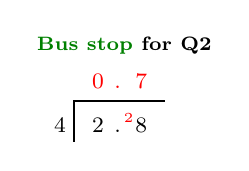
\begin{tikzpicture}[every node/.style={font=\scriptsize}]
\begin{scope}[xshift=0.6cm]
\node[dhead] at (-0.6,1.1) {\ealkey{Bus stop} for Q2};
\busframe{4}{1.15}
\foreach \x/\d in {0.3/2, 0.55/., 0.85/8} \node[bsd] at (\x,0) {$\d$};
\foreach \x/\d in {0.3/0, 0.55/., 0.85/7} \node[bsa] at (\x,0.55) {$\d$};
\node[bscarry] at ({0.85-0.16},0.12) {$2$};
\end{scope}
\end{tikzpicture}

\column{0.68\textwidth}
\vspace{-1.5em}
\footnotesize
\begin{enumerate}\setcounter{enumi}{0}\tightlist
  \item \ealpara{Wykonaj każde obliczenie, a następnie użyj go, aby \ealkeytr{rozwiązać} \ealkeytr{równanie} obok.}{}
  \instr{Work out each calculation, then use it to \ealkey{solve} the \ealkey{equation} beside it.}
  \begin{subqs}
  \begin{multicols}{2}
    \item $-18\div3=$\ashow{$-6$}
    \item $2.8\div4=$\ashow{$0.7$}
    \item $6\div0.5=$\ashow{$\tfrac{60}{5}=12$}
    \columnbreak
    \item $3x=-18$ \ashow{$x=-6$}
    \item $4x=2.8$ \ashow{$x=0.7$}
    \item $0.5x=6$ \ashow{$x=12$}
  \end{multicols}
  \end{subqs}
  \item \ealpara{W $4x=2.8$, $4$ jest \ablank{\ealkeytr{współczynnikiem}} $x$.}{In $4x=2.8$, the $4$ is the \ablank{\ealkey{coefficient}} of $x$.}
\end{enumerate}
\end{columns}
\end{frame}

\begin{frame}[t]{Starter 6: \ealkey{One-Step Equations} (2 of 3)}
\footnotesize
\begin{enumerate}\setcounter{enumi}{2}\tightlist
  \item \ealpara{Zakreśl \ealkeytr{działanie}, które jest \ealkeytr{wektorem przeciwnym} do:}{}
  \instr{Circle the \ealkey{operation} that is the \ealkey{reverse} of:}
  \begin{subqs}
    \item \ealpara{mnożenie}{}\makebox[2.2cm][l]{multiplication} \circleops{4}{}
    \item \ealpara{dzielenie}{}\makebox[2.2cm][l]{division} \circleops{3}{}
  \end{subqs}
  \item \ealpara{\ealkeytr{Rozwiąż} każde \ealkeytr{równanie}.}{}
  \instr{\ealkey{Solve} each \ealkey{equation}.}
  \begin{subqs}
  \begin{multicols}{2}
    \item $-2x=10$ \ashow{$x=-5$}
    \columnbreak
    \item $\dfrac{x}{5}=-2$ \ashow{$x=-10$}
  \end{multicols}
  \end{subqs}
\end{enumerate}
\end{frame}

\begin{frame}[t]{Starter 6: \ealkey{One-Step Equations} (3 of 3)}
\footnotesize
\begin{enumerate}\setcounter{enumi}{4}\tightlist
  \item \ealpara{Pięciu przyjaciół dzieli rachunek po równo i każdy płaci \pounds7.40. \ealkeytr{Rozwiąż} \ealkeytr{równanie}, aby znaleźć rachunek, \pounds$b$.}{Five friends share a bill equally, and each pays \pounds7.40. \ealkey{Solve} an \ealkey{equation} to find the bill, \pounds$b$.}
        \ashow{$\tfrac{b}{5}=7.40$, \; $b=37$}
  \item \ealpara{Zapisz \ealkeytr{równanie} z \ealkeytr{rozwiązaniem} $x=-0.5$:}{}
  \instr{Write an \ealkey{equation} with the \ealkey{solution} $x=-0.5$:}
  \begin{subqs}
  \begin{multicols}{2}
    \item \ealpara{(Wyzwanie) gdzie $x$ jest pomnożone przez liczbę}{(Challenge) where $x$ is multiplied by a number} \ashow{For example $4x=-2$}
    \columnbreak
    \item \ealpara{(Wyzwanie) gdzie $x$ jest podzielone przez liczbę}{(Challenge) where $x$ is divided by a number} \ashow{For example $\tfrac{x}{2}=-0.25$}
  \end{multicols}
  \end{subqs}
\end{enumerate}
\end{frame}

\begin{frame}[t]{Starter 7: \ealkey{Two-Step Equations} (1 of 3)}
\footnotesize
\begin{enumerate}\setcounter{enumi}{0}\tightlist
\begin{multicols}{2}
  \item $1-9=$\ashow{$-8$}
  \columnbreak
  \item $-8\div4=$\ashow{$-2$}
\end{multicols}
  \item \ealpara{W $3n+4=19$, lewa strona jest \ablank{\ealkeytr{wyrażeniem}}.}{In $3n+4=19$, the left-hand side is an \ablank{\ealkey{expression}}.}
\end{enumerate}
\end{frame}

\begin{frame}[t]{Starter 7: \ealkey{Two-Step Equations} (2 of 3)}
\begin{columns}[T,onlytextwidth]
\column{0.32\textwidth}
\vspace{-0.4em}
\bothsides{Working for Q6}{3n+4 \& = \& 19\\ 3n \& = \& \ablank{15}\\
  n \& = \& \ablank{5}\\}{-4, \div3}

\column{0.68\textwidth}
\vspace{-1.5em}
\footnotesize
\begin{enumerate}\setcounter{enumi}{3}\tightlist
  \item \ealpara{Zakreśl \ealkeytr{działanie}, które jest \ealkeytr{wektorem przeciwnym} do:}{}
  \instr{Circle the \ealkey{operation} that is the \ealkey{reverse} of:}
  \begin{subqs}
    \item \ealpara{dodawanie $4$}{}\makebox[2.6cm][l]{adding $4$} \circleops{2}{4}
    \item \ealpara{mnożenie przez $3$}{}\makebox[2.6cm][l]{multiplying by $3$} \circleops{4}{3}
  \end{subqs}
  \item \ealpara{Myślę o liczbie, $n$. Mnożę ją przez $3$ i dodaję $4$, i otrzymuję $19$. Zapisz \ealkeytr{równanie}, a następnie uzupełnij obliczenia po lewej.}{I think of a number, $n$. I multiply it by $3$ and add $4$, and I get $19$. Write an \ealkey{equation}, then complete the working on the left.}
        \ashow{$3n+4=19$}
  \item \ealpara{Sprawdź odpowiedź do Q6, \ealkeytr{podstawiając} ją do $3n+4$.}{Check your answer to Q6 by \ealkey{substituting} it into $3n+4$.}
        \ashow{$3\times5+4=19$ \checkmark}
\end{enumerate}
\end{columns}
\end{frame}

\begin{frame}[t]{Starter 7: \ealkey{Two-Step Equations} (3 of 3)}
\begin{columns}[T,onlytextwidth]
\column{0.32\textwidth}
\vspace{-0.4em}
\bothsides{Working for Q10}{4x+9 \& = \& 1\\ 4x \& = \& \ablank{-8}\\
  x \& = \& \ablank{-2}\\}{-9, \div4}

\column{0.68\textwidth}
\vspace{-1.5em}
\footnotesize
\begin{enumerate}\setcounter{enumi}{6}\tightlist
  \item \ealpara{\ealkeytr{Rozwiąż} każde \ealkeytr{równanie}.}{}
  \instr{\ealkey{Solve} each \ealkey{equation}.}
  \begin{subqs}
  \begin{multicols}{2}
    \item $2x+5=11$ \ashow{$2x=6$, \; $x=3$}
    \columnbreak
    \item $5x-3=17$ \ashow{$5x=20$, \; $x=4$}
  \end{multicols}
  \begin{multicols}{2}
    \item \ealpara{$4x+9=1$, z obliczeniami po lewej}{$4x+9=1$, with the working on the left}
    \columnbreak
    \item $2x-1=6$ \ashow{$2x=7$, \; $x=3.5$}
  \end{multicols}
  \end{subqs}
  \item \ealpara{Hydraulik pobiera opłatę za wezwanie \pounds20 i \pounds35 za godzinę. Rachunek wynosi \pounds125. \ealkeytr{Rozwiąż} \ealkeytr{równanie}, aby znaleźć liczbę godzin, $h$.}{A plumber charges a \pounds20 call-out fee and \pounds35 an hour. A bill is \pounds125. \ealkey{Solve} an \ealkey{equation} to find the number of hours, $h$.}
        \ashow{$35h+20=125$, \; $h=3$}
  \item \ealpara{(Wyzwanie) \ealkeytr{Rozwiąż} $x+2x+3=18$.}{(Challenge) \ealkey{Solve} $x+2x+3=18$.}
        \ashow{$3x+3=18$, \; $x=5$}
\end{enumerate}
\end{columns}
\end{frame}

\begin{frame}[t]{Starter 8: \ealkey{Decimals} \& \ealkey{Negatives} in \ealkey{Equations} (1 of 3)}
\footnotesize
\begin{enumerate}\setcounter{enumi}{0}\tightlist
\begin{multicols}{2}
  \item $3+1.2=$\ashow{$4.2$}
  \columnbreak
  \item $4.2\div2=$\ashow{$2.1$}
\end{multicols}
  \item \ealpara{W $2x-1.2=3$, \ealkeytr{współczynnik} $x$ wynosi \ablank{$2$}, a \ealkeytr{stała} po lewej stronie wynosi \ablank{$-1.2$}.}{In $2x-1.2=3$, the \ealkey{coefficient} of $x$ is \ablank{$2$}, and the \ealkey{constant} on the left-hand side is \ablank{$-1.2$}.}
\end{enumerate}
\end{frame}

\begin{frame}[t]{Starter 8: \ealkey{Decimals} \& \ealkey{Negatives} in \ealkey{Equations} (2 of 3)}
\begin{columns}[T,onlytextwidth]
\column{0.34\textwidth}
\vspace{-0.4em}
\bothsides{Working for Q6}{2x-1.2 \& = \& 3\\ 2x \& = \& \ablank{4.2}\\
  x \& = \& \ablank{2.1}\\}{\ablank{+1.2}, \ablank{\div2}}

\column{0.66\textwidth}
\vspace{-1.5em}
\footnotesize
\begin{enumerate}\setcounter{enumi}{3}\tightlist
  \item \ealpara{Zakreśl \ealkeytr{działanie}, które jest \ealkeytr{wektorem przeciwnym} do:}{}
  \instr{Circle the \ealkey{operation} that is the \ealkey{reverse} of:}
  \begin{subqs}
    \item \ealpara{odejmowanie $1.2$}{}\makebox[2.3cm][l]{subtracting $1.2$} \circleops{1}{1.2}
    \item \ealpara{mnożenie przez $2$}{}\makebox[2.3cm][l]{multiplying by $2$} \circleops{4}{2}
  \end{subqs}
  \item \ealpara{\ealkeytr{Rozwiąż} $2x-1.2=3$. Zapisz \ealkeytr{działania} obok strzałek.}{\ealkey{Solve} $2x-1.2=3$. Write the \ealkey{operations} beside the arrows.}
  \item \ealpara{\ealkeytr{Rozwiąż} każde \ealkeytr{równanie}.}{}
  \instr{\ealkey{Solve} each \ealkey{equation}.}
  \begin{subqs}
  \begin{multicols}{2}
    \item $3x+8=-7$ \ashow{$3x=-15$, \; $x=-5$}
    \columnbreak
    \item $\dfrac{x}{2}+3=-1$ \ashow{$\tfrac{x}{2}=-4$, \; $x=-8$}
  \end{multicols}
  \begin{multicols}{2}
    \item $5x-2.5=10$ \ashow{$5x=12.5$, \; $x=2.5$}
    \columnbreak
    \item $0.5x+4=1$
          \ashow{$0.5x=-3$, \; $x=\tfrac{-3}{0.5}=\tfrac{-30}{5}=-6$}
  \end{multicols}
  \end{subqs}
\end{enumerate}
\end{columns}
\end{frame}

\begin{frame}[t]{Starter 8: \ealkey{Decimals} \& \ealkey{Negatives} in \ealkey{Equations} (3 of 3)}
\begin{columns}[T,onlytextwidth]
\column{0.34\textwidth}
\vspace{-0.4em}
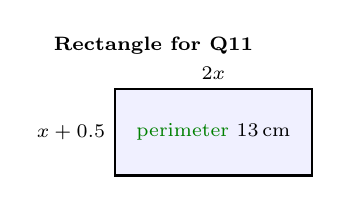
\begin{tikzpicture}[every node/.style={font=\scriptsize}]
\node[dhead] at (0,1.65) {Rectangle for Q11};
\rect{2x}{x+0.5}{\ealkey{perimeter} $13$\,cm}
\end{tikzpicture}

\column{0.66\textwidth}
\vspace{-1.5em}
\footnotesize
\begin{enumerate}\setcounter{enumi}{6}\tightlist
  \item \ealpara{Zapisz \ealkeytr{równanie} na \ealkeytr{obwód} \ealkeytr{prostokąta} i je \ealkeytr{rozwiąż}.}{Write an \ealkey{equation} for the \ealkey{perimeter} of the \ealkey{rectangle}, and \ealkey{solve} it.}
        \ashow{$6x+1=13$, \; $x=2$}
  \item \ealpara{(Wyzwanie) Zapisz \ealkeytr{równanie dwuetapowe} z \ealkeytr{rozwiązaniem} $x=-0.5$.}{(Challenge) Write a \ealkey{two-step equation} with the \ealkey{solution} $x=-0.5$.}
        \ashow{For example $2x+3=2$}
\end{enumerate}
\end{columns}
\end{frame}

\end{document}